\documentclass[12pt,letterpaper]{article}
\usepackage[latin1]{inputenc}
\usepackage[spanish]{babel}
\usepackage{graphicx}
\usepackage[left=2cm,right=2cm,top=2cm,bottom=2cm]{geometry}
\usepackage{graphicx} % figuras
\usepackage{subfigure} % subfiguras
\usepackage{float} % para usar [H]
\usepackage{amsmath}
\usepackage{txfonts}
\usepackage{stackrel} 
\usepackage[latin1]{inputenc}
\usepackage{multirow}
\usepackage{enumerate} % enumerados
\renewcommand{\labelitemi}{$-$}
\renewcommand{\labelitemii}{$\cdot$}
\author{Fanny Clemente}
\title{Caratula}
\begin{document}



\author{Fanny Clemente}
\title{Caratula}

\begin{titlepage}
\begin{center}
\large{UNERSIDAD PRIVADA DE TACNA}\\
\vspace*{-0.025in}
\begin{figure}[htb]
\begin{center}

\includegraphics[width=8cm]{./IMAGENES/logo}
\end{center}
\end{figure}
\vspace*{0.15in}
INGENIERIA DE SISTEMAS  \\

\vspace*{0.5in}
\begin{large}
TITULO:\\
\end{large}

\vspace*{0.1in}
\begin{Large}
\textbf{Laboratorio07} \\
\end{Large}

\vspace*{0.3in}
\begin{Large}
\textbf{CURSO:} \\
\end{Large}

\vspace*{0.1in}
\begin{large}
BASE DE DATOS II\\
\end{large}

\vspace*{0.3in}
\begin{Large}
\textbf{DOCENTE(ING):} \\
\end{Large}

\vspace*{0.1in}
\begin{large}
 Patrick Cuadros Quiroga\\
\end{large}

\vspace*{0.2in}
\vspace*{0.1in}
\begin{large}
Integrantes: \\
\begin{flushleft}
Acevedo Vásquez, Leonardo Fernando 	(2014047512) \\
Andía Bernedo, Josei Jomar 			(2014049093) \\
Condori Velarde, Sonia          	(2014049546) \\
Clemente Cruz, Fanny Luz    		(2014049550) \\
Flores Colque, Gisela           	(2014049547) \\
Llatasi Cohaila, Cristian Omar		(2014037546) \\
Morales Anquise, Tommy Edwards 		(2015050480) \\
Ticona Arcaya, Sergio Alexis		(2014049171) \\
Tapia Ticona, Lupe Carolina			(2014049548) \\
\end{flushleft}
\end{large}
\end{center}

\end{titlepage}




 \tableofcontents
 \newpage
SESI0N DE LABORATORIO N° 07:
Instalacion de Oracle Database 12c

 
\section{Objetivos} 

\begin{enumerate}[1.]
    \item Brindar al estudiante los conocimientos necesarios para realizar la Instalacion de un servidor de Base de Datos
Oracle sobre un sistema operativo Linux dentro de un contenedor de Docker.
    
   \item Otorgar al estudiante los conocimientos necesarios para realizar la instalacion de este servidor dentro de un
ambiente contenerizado.
		\end{enumerate} 
		


\section{Requerimientos} 
\subsection{Mapping Entities and Atributes}
\subsubsection{Ejercicio 1: Creacion de un Glosario a Partir del Modelo Logico.} 
descripcion general  \\
En esta practica, creara un glosario a partir del modelo logico de la base de datos academica. \\

Tareas\\
\begin{enumerate}[1.]
    \item  Conocimientos\\ \\
Para el desarrollo de esta práctica se requerira de los siguientes conocimientos básicos:\\
- Conocimientos basicos de comandos a nivel de consola o terminal de texto.\\
- Conocimientos basicos de redes locales.
     
    \item Hardware\\
Se necesitará un PC (computadora personal), con las siguientes características:\\
- 01 procesador de doble núcleo o superior\\
- 6Gb de memoria física (RAM) o superior\\
- Disco duro con 100Gb de capacidad y al menos 30Gb de espacio libre\\
- Unidad Lector de DVD.\\
- Interfaz de Red Ethernet activa\\
    
    \item Software\\
Asimismo, se necesita los siguientes aplicativos:\\
- Windows 10 o superior preinstalado, de preferencia actualizado con todos los parches de seguridad.\\
- Característica Hyper-V activada\\

    \begin{center}
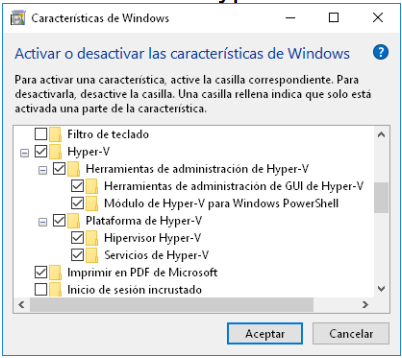
\includegraphics[width=15cm]{./IMAGENES/img1}
\end{center}

- Docker for Windows preinstalado

\begin{center}
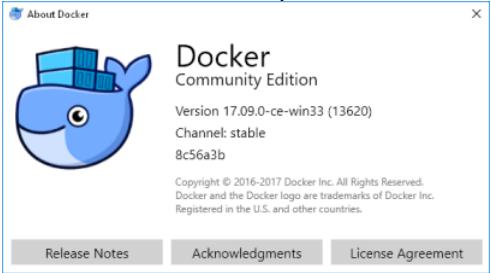
\includegraphics[width=15cm]{./IMAGENES/img2}
\end{center} 
- Contenedor de Oracle Database 12c (archivo de extension .tar).
		\end{enumerate}





 \newpage
\subsection{CONSIDERACIONES INICIALES}

\begin{enumerate}[1.]
    \item Docker debe estar configurado para utilizar al menos 4Gb de memoria RAM.
Liberar los puertos 1521 y 5500 del Firewall de Windows.
    	
		\item De preferencia copiar en una unidad distinta a la del sistema operativo el archivo con extension .tar.
\item Liberar los puertos 1521 y 5500 del Firewall de Windows.
		\end{enumerate}


 
\section{DESARROLLO } 

\begin{enumerate}[1.]
    \item  PASO 1.- Abrir el terminal de PowerShell como Administrador. 
     \begin{center}
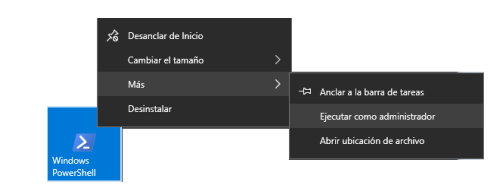
\includegraphics[width=15cm]{./IMAGENES/img3}
\end{center} 
    \item PASO 2.- Acceder a la ruta donde se encuentra el archivo con extension .tar. (La ruta dependerá de donde se haya
almacenado el archivo de extension .tar)
\begin{center}
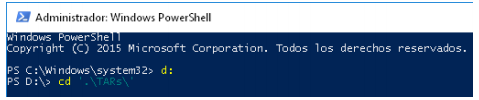
\includegraphics[width=15cm]{./IMAGENES/img4}
\end{center} 

\item Ejecutar el siguiente comando. \\
\begin{center}
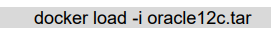
\includegraphics[width=15cm]{./IMAGENES/img11}
\end{center} 
El cual realiza la carga de la imagen del contenedor hacia Docker.
\begin{center}
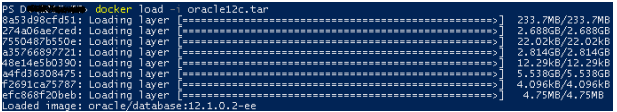
\includegraphics[width=15cm]{./IMAGENES/img5}
\end{center} 

\item PASO 4.- Ejecutar el siguiente comando.
 \\
 \begin{center}

\includegraphics[width=15cm]{./IMAGENES/img12}
\end{center} 

El cual permite visualizar las imágenes de contenedores cargadas en Docker.
\begin{center}
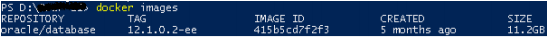
\includegraphics[width=15cm]{./IMAGENES/img6}
\end{center} 
\item PASO 5.- Ejecutar el siguiente comando.
 \\
\begin{center}
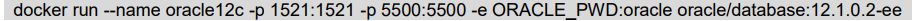
\includegraphics[width=15cm]{./IMAGENES/img13}
\end{center} 
El cual realiza la ejecucion de la imagen del contenedor en una nueva instancia del sistema gestor de base de
datos relacional Oracle 12c.
\begin{center}
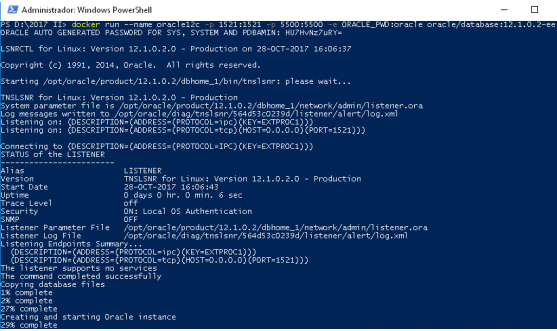
\includegraphics[width=15cm]{./IMAGENES/img7}
\end{center} 
\item PASO 6.- De ser todo correcto, iniciar un navegador de internet (Chrome, Mozzila, IE, etc.) y colocar la siguiente URL en la barra de
direcciones.
 \\
\begin{center}

\includegraphics[width=15cm]{./IMAGENES/img8}
\end{center} 
Debe visualizar el administrador empresarial (Enterprise Manager). En algunos navegadores es necesario
utilizar la opcion Acceder a sitio no seguro.
\begin{center}
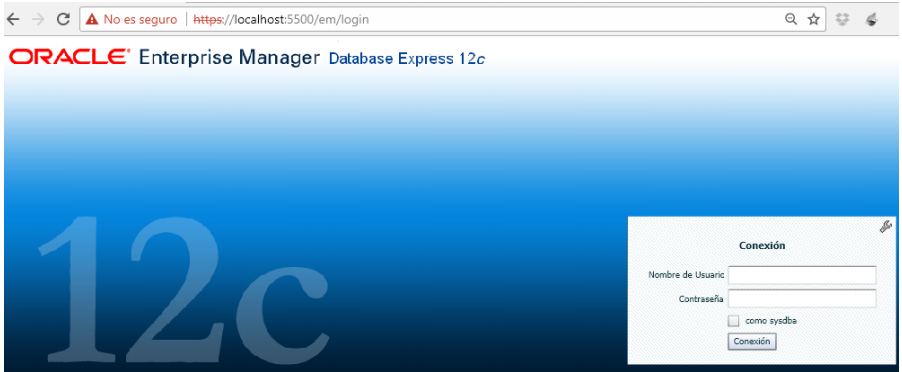
\includegraphics[width=15cm]{./IMAGENES/img9}
\end{center} 

\item PASO 7.- Iniciar sesion con el usuario SYS y la clave establecida anteriormente.
\begin{center}
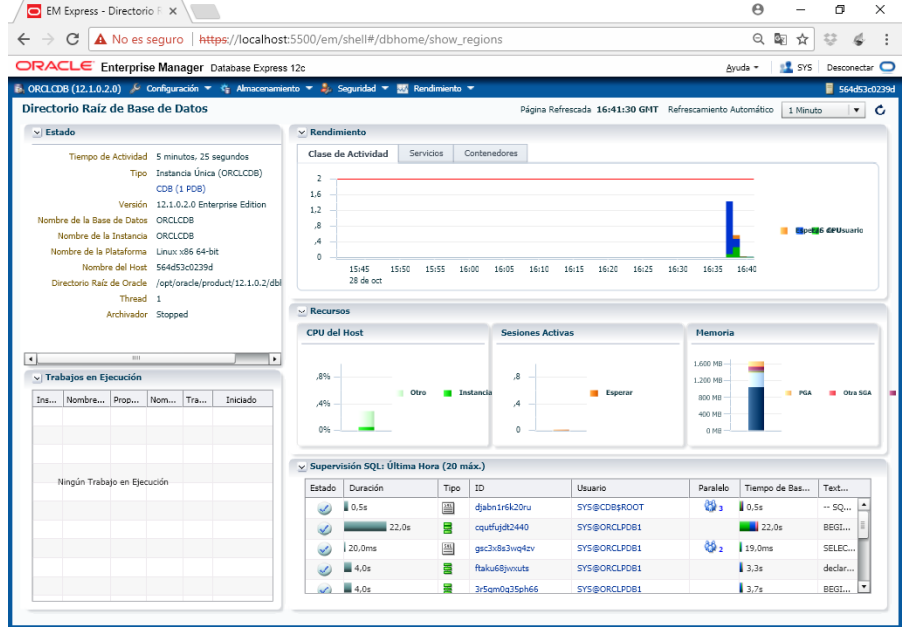
\includegraphics[width=15cm]{./IMAGENES/img10}
\end{center} 
		\end{enumerate}


\section{CUESTIONARIO } 

\begin{enumerate}[1.]
    \item  Para que sirven cada una de las opciones del comando docker siguiente:
     
    \item ¿Con que comandos Docker puedo: a) Detener o finalizar un contenedor. b)Eliminar una
imagen?
a) Para detener o finalizar un contenedor utilizamos el comando  docker stop



\item Ejecute nuevamente el comando Docker para crear una nueva instancia del SGBDR Oracle
12c (un nuevo contenedor distinto a oracle12c) redireccionando el puerto del Listener al 1523
y el puerto del Enterprise Manager al 8181. Capture los resultados



\item ¿Con qué usuario(s) puedo conectarme al servidor a través del Administrador Empresarial?

\item ¿Qué es el Listener? ¿Para qué se utiliza?


		\end{enumerate}


\section{Referencias Electronicas } 

-Sitio oficial de contenedores Docker para Oracle Database\\
https://github.com/oracle/docker-images/tree/master/OracleDatabase\\ \\
- Activando Hyper-V como inicio alternativo en Windows 10.\\
http://patrickcuadros.blogspot.pe/2016/11/configurando-una-de-inicio-de-windows.html



\end{document}
